
\documentclass{article}

\usepackage[version=3]{mhchem} % Package for chemical equation typesetting
\usepackage{siunitx} % Provides the \SI{}{} and \si{} command for typesetting SI units
\usepackage{graphicx} % Required for the inclusion of images
\usepackage{natbib} % Required to change bibliography style to APA
\usepackage{amsmath} % Required for some math elements 
\usepackage{caption}
\usepackage{subcaption}
\usepackage{listings}
\usepackage{color}
 
\definecolor{codegreen}{rgb}{0,0.6,0}
\definecolor{codegray}{rgb}{0.5,0.5,0.5}
\definecolor{codepurple}{rgb}{0.58,0,0.82}
\definecolor{backcolour}{rgb}{0.95,0.95,0.92}
 
\lstdefinestyle{mystyle}{
    backgroundcolor=\color{backcolour},   
    commentstyle=\color{codegreen},
    keywordstyle=\color{codepurple},
    numberstyle=\tiny\color{codegray},
    stringstyle=\color{codepurple},
    basicstyle=\footnotesize,
    breakatwhitespace=false,         
    breaklines=true,                 
    captionpos=b,                    
    keepspaces=true,                 
    numbers=left,                    
    numbersep=5pt,                  
    showspaces=false,                
    showstringspaces=false,
    showtabs=false,                  
    tabsize=2
}
\lstset{style=mystyle}

\setlength\parindent{0pt} % Removes all indentation from paragraphs

\renewcommand{\labelenumi}{\alph{enumi}.} % Make numbering in the enumerate environment by letter rather than number (e.g. section 6)

\newcommand\tab[1][0.5cm]{\hspace*{#1}}

%\usepackage{times} % Uncomment to use the Times New Roman font

\renewcommand{\thesubsection}{\thesection.\alph{subsection}}

%----------------------------------------------------------------------------------------
%	DOCUMENT INFORMATION
%----------------------------------------------------------------------------------------

\title{COMP 304: Assignment 2} % Title

\author{Berkay \textsc{Barlas}} % Author name

\date{\today} % Date for the report

\begin{document}

\maketitle % Insert the title, author and date

\begin{center}
\begin{tabular}{l r}
Date Performed: & April 15, 2019 \\ % Date the experiment was performed
Instructor: & Didem Unat % Instructor/supervisor
\end{tabular}
\end{center}

% If you wish to include an abstract, uncomment the lines below
% \begin{abstract}
% Abstract text
% \end{abstract}

%----------------------------------------------------------------------------------------
%	SECTION 1
%----------------------------------------------------------------------------------------


\section{Problem 1}

\subsection{}

\begin{description}
    \item[Process Execution Gantt Chart of FCFS] \hfill 
    
    
    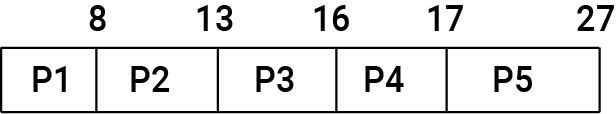
\includegraphics[width=1\linewidth]{./fcfs.png}
    \item[Process Execution Gantt Chart of SJF] \hfill 
    
    
    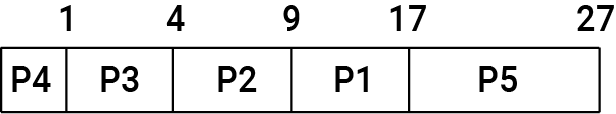
\includegraphics[width=1\linewidth]{./sjf.png}
    \item[Process Execution Gantt Chart of non-preemptive Priority] \hfill 
    
    
    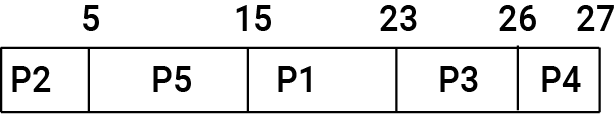
\includegraphics[width=1\linewidth]{./priority.png}
    \item[Process Execution Gantt Chart of RR] \hfill 
    
    
    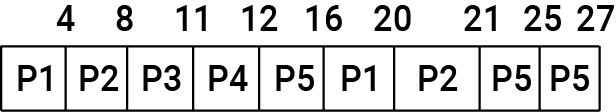
\includegraphics[width=1\linewidth]{./rr.png}
\end{description}

\subsection{} If the context-switch overhead is 1 ms, calculate the waiting time of each process for
each of the scheduling algorithms in part (a). Which of the schedules results in the minimal
average waiting time? 

SJF(Shortest Job First) results in the minimal average waiting time.\\ \\

\begin{description}
    \item[Process Execution Gantt Chart of FCFS] \hfill 
    \begin{description}
        \item[Waiting Time of P1:] 0
        \item[Waiting Time of P2:] 9 
        \item[Waiting Time of P3:] 15
        \item[Waiting Time of P4:] 19
        \item[Waiting Time of P5:] 21
        \item[Average waiting time:] ( 9 + 15 + 19 + 21 ) / 5 = 12,8
    \end{description}
    \item[Process Execution Gantt Chart of SJF] \hfill 
    \begin{description}
        \item[Waiting Time of P1:] 12
        \item[Waiting Time of P2:] 6 
        \item[Waiting Time of P3:] 2
        \item[Waiting Time of P4:] 0
        \item[Waiting Time of P5:] 21
        \item[Average waiting time:] ( 12 + 6 + 2 + 0 + 21 ) / 5 = 8.2 
    \end{description}
    \item[Process Execution Gantt Chart of non-preemptive Priority] \hfill 
    \begin{description}
        \item[Waiting Time of P1:] 17
        \item[Waiting Time of P2:] 0 
        \item[Waiting Time of P3:] 26
        \item[Waiting Time of P4:] 30
        \item[Waiting Time of P5:] 6
        \item[Average waiting time:] ( 17 + 0 + 26 + 30 + 6) / 5 = 15,8 
    \end{description} 
    
    \item[Process Execution Gantt Chart of RR] \hfill 
    \begin{description}
        \item[Waiting Time of P1:] 16 + 5 - 8 = 13
        \item[Waiting Time of P2:] 21 + 6 - 5 = 22
        \item[Waiting Time of P3:] 10
        \item[Waiting Time of P4:] 14 
        \item[Waiting Time of P5:] 27 + 8 -10 = 25
        \item[Average waiting time:] (13 + 22 + 10 + 14 + 25) / 5 = 16,8
    \end{description}
    
\end{description}

\subsection{Calculate average turnaround time for each of the scheduling algorithms in part (a).}
\begin{description}
    \item[Average turnaround time for FCFS] \hfill 
\\( 8 + 13 + 16 + 17 + 27 ) / 5 = 16.2
    \item[Average turnaround time for SJF] \hfill 
\\( 1 + 4 + 9 + 17 + 27 ) / 5 = 11.6   
    \item[Average turnaround time for non-preemptive Priority] \hfill 
\\( 5 + 15 + 23 + 26 + 27 ) / 5 = 19.2  
    \item[Average turnaround time for RR] \hfill 
\\( 20 + 21 + 11 + 12 + 27 ) / 5 = 18.2
\end{description}

\section{Problem 2}
Now assume that the context-switching overhead is equivalent to 0.5 ms. Calculate the CPU utilisation for all four scheduling algorithms in Problem 1.
\\ 
\begin{equation*}
    CPU utilisation  = 100 * \frac{{Total Time Spend on Processes}}{\mathrm{Total Time Spend on Execution}}
%\begin{center}\ce{}\end{center}
\end{equation*}
\begin{description}
    \item[CPU utilisation of FCFS] \hfill \\ 
(27 / 29 * 100) = 93,10
    \item[CPU utilisation of SJF] \hfill \\
    (27 / 29 * 100) = 93,10
    \item[CPU utilisation of non-preemptive Priority] \hfill \\
    (27 / 29 * 100) = 93,10
    \item[CPU utilisation of RR] \hfill \\
(27 / 31 * 100) = 87,09
\end{description}

\section{Problem 3}

\subsection{}
\tab There is race condition in code, thus, output is non-deterministic and depends on order of process execution.
\\The available\_connections is shared variable and it might be written by multiple threads simultaneously inside of the connect() and disconnect() methods.
\\Since write is actually consist of multiple Instructions, a race condition may occur when two or more threads access the shared data and they try to change it at the same time.
\subsection{}
We could use locks to prevent race condition.

\begin{lstlisting}[language=C]
//PROBLEM 3
#define MAX_CONNECTIONS 5000
int available_connections = MAX_CONNECTIONS;
mutex lock;

/* When a thread wishes to establish a connection with the rver,
it invokes the connect() function:*/

int connect() {
    mutex_lock(&lock); 
    if (available_connections < 1) {
        mutex_unlock(&lock);
        return -1;
    } else {
        available_connections--;
    }
    mutex_unlock(&lock);
    return 0;
}

 /* When a thread wishes to drop a connection with the server,
 it invokes disconnect() */
 int disconnect() {
    mutex_lock(&lock);
    available_connections++;
    mutex_unlock(&lock);
    return 0;
 }
\end{lstlisting}

\subsection{}
\tab 
\\ \tab Using atomic integer will prevent the race condition that caused by change of shared variable by multiple threads at the same time. However, replacing the integer with atomic integer is not enough. While one of the threads inside of the if statement of connect method (before returning) another thread might increase the available\_connections variable which might effect of the result of if statement. For example, connect() method could return \-1 even available\_connections is 1 (It was 0 when the statement checked but then inreased to 1 before return by another thread inside of the disconnect() method. ).
\newpage
\section{Problem 4}
\tab We could use semaphore with initial value M ,however, if a party with more than 4 numcustomers arrive we need to be sure we have enough rooms. Thus, we can use a semaphore with initial value 1 and a global variable to check available number of rooms.
\begin{lstlisting}[language=C]

    semaphore roomLock = 1;
    int roomNum = M;

    int makeReservation(int numCustomers) {
        int roomNeeded = (numCustomers + 3 ) / 4;  
        // I added 3 to round upper bound. 
        // When 1 || 2 || 3 || 4 customer come roomNeeded should be 1 
        // When 5 customer come roomNeeded should be 2 
        // int a = (2 + 3) / 4 = 1; a = 1
        wait(roomLock);
        
        if(roomNum >=roomNeeded ) {
            //accept
            roomNum = roomNum - roomNeeded;

        } else {
            //decline
        }
        signal(roomLock);
        return 0;
    }

    int checkout(int roomNumber) {
        wait(roomLock);
        roomNum = roomNum + roomNumber;
        signal(roomLock);
    }

\end{lstlisting}
\newpage
\section{Problem 5}
\tab I we can use 3 different semaphores with initial value 1 for each data item. Process P and S requires only one semaphore since they only share single data item with other process. However, processes Q and R share two data item therefore they need 2 semaphores. 
\begin{lstlisting}[language=C]

    data d1; // shared data item, could be any data
    data d2; // shared data item, could be any data
    data d3; // shared data item, could be any data
    semaphore lock1 = 1;
    semaphore lock2 = 1;
    semaphore lock3 = 1;
/* process P runs in this function */
void *P() {
    wait(lock1);

    //makeCalculation

    signal(lock1);
}
 
/* process Q runs in this function */
void *Q() {
    wait(lock2);
    wait(lock1);

    //makeCalculation

    signal(lock1);
    signal(lock2);
}

/* process R runs in this function */
void *R() {
    wait(lock2);
    wait(lock3);

    //makeCalculation

    signal(lock3);
    signal(lock2);
}

/* process S runs in this function */
void *S() {
    wait(lock3);

    //makeCalculation

    signal(lock3);
}
\end{lstlisting}
\end{document}